%\documentclass{beamer}
%\documentclass[notes=only]{beamer}   % only notes
\documentclass{beamer}              % only frames

\usetheme{simple}

\usepackage{lmodern}
\usepackage[scale=2]{ccicons}
\usepackage[T2A]{fontenc}
\usepackage[utf8]{inputenc}  
\usepackage[russian]{babel}
\usepackage{listings}
\usepackage{geometry}
\usepackage{marginnote}
\usepackage{movie15}
  
% TODO: 
%   position adjustement
%   change colours
%       

% Watermark background (simple theme)

%\setwatermark[hoffset=2cm,voffset=1,5cm]{
\includegraphics[height=8cm]{img/watermark1.png}}
\setwatermark{
\includegraphics[height=9cm]{img/watermark1.png}}


\title{Поиск программ для ПЛИС с помощью профилирования и эмуляции}
\subtitle{}
\date{\today}
\author{Баглий Антон}
\institute{\url{sfedu.ru}}

\begin{document}

\maketitle


\begin{frame}{поиск частей программ для отображения на ПЛИС}
  \framesubtitle{}
   
  \begin{columns}
    \column{.7\textwidth}
      \begin{itemize}
        \item Программы (или циклы), которые нужно ускорить
        \item Схемы для которых поместятся на ПЛИС
        \item Схемы для которых эффективно используют ресурсы
        \item Которые получат достаточное ускорение (с учетом памяти и т.п.)
      \end{itemize}

    \column{.3\textwidth}
      \begin{block}{В общем}
         Множество конфликтующих требований и факторов, влияющих на производительность
      \end{block}
  \end{columns}		  
\end{frame}

\begin{frame}{поиск частей программ для отображения на ПЛИС}
  \framesubtitle{выбор ограниченных участков}
   
  \begin{columns}
    \column{.7\textwidth}
      \begin{itemize}
        \item Повторяющиеся группы операторов или выражения
        \item Такие операторы, которые наш компилятор сможет конвейеризовать
        \item Похожие выражения, по которым можно построить общий ковейер
      \end{itemize}

    \column{.3\textwidth}
      \begin{block}{Для чего}
         Можно быстро оценить перспективы программы для ПЛИС (исследование пространства возможных характеристик) за счет расширяемых архитектур IP-ядер и добавления инструкций к ним.
      \end{block}
  \end{columns}		  
\end{frame}

\begin{frame}[fragile]
\frametitle{Метрики кода и поверхностный статический анализ}
  \framesubtitle{Может ли это работать}
  \begin{columns}
    \column{.4\textwidth}
      \begin{itemize}
        \item Быстро работает
        \item Легко реализовать
      \end{itemize}
      
      \begin{block}{Поверхностный анализ}
         Тяжело получить хороший результат. Возможно накопление базы для применения методов машинного обучения (комп. статистики)
      \end{block}

    \column{.6\textwidth}
      
      
% TODO: хороший пример      
\begin{lstlisting}[frame=single]
 for (int i = 0; i < N; i++) {
   for (int j = 0; j < M; j++) {
      A = A*2;
   }
 }
\end{lstlisting}
\label{clone_listing}
      
  \end{columns}
  
\end{frame}

\begin{frame}[fragile]
\frametitle{Поиск специальных гнезд циклов}
  \framesubtitle{}
  \begin{table}
    \begin{tabular}{ | p{1.5cm} | p{2cm} | p{1cm} | p{6cm} |}
    \hline
    Программа & долго счит. & интересных & особенности \\ \hline
    adpcm & 3 & 0 & нельзя заранее определить число итераций \\ \hline
    aes & 3 & 1 &  \\ \hline
    blowfish & 1 & 0 & цикл уже полностью развернут в исходном коде \\ \hline
    dfadd & 1 & 0 &  \\ \hline
    dfdiv & 1 & 0 &  \\ \hline
    dfmul & 1 & 0 &  \\ \hline
    dfsin & 1 & 0 &  \\ \hline
    gsm & 1 & 0 &  \\ \hline
    jpeg & 4 & 2 & нельзя заранее определить число итераций \\ \hline
    mips & 1 & 1 & нельзя заранее определить число итераций \\ \hline
    motion & 2 & 0 &  \\ \hline
    sha & 1 & 0 &  \\ \hline
    \end{tabular} 
    \caption{Результаты поиска специальных циклов в бенчмарках CHStone}
    \label{table:CHStoneSingularLoops}
\end{table}
\end{frame}

\begin{frame}[fragile]
\frametitle{Статическое профилирование}
  \framesubtitle{}
  \begin{columns}
    \column{.5\textwidth}
        \begin{itemize}
            \item Быстрый анализ 
            \item Неточный
            \item Работает на простых примерах
        \end{itemize}      

    \column{.5\textwidth}
    \begin{block}{Не подходит для ПЛИС?}
         Простой подсчет числа операций очевидно не дает оценки характеристик конвейера.
         Полезным может быть только оценка интенсивности обмена с памятью
      \end{block}
    \label{encode_listing}
      
\end{columns}
  
\end{frame}

\begin{frame}[fragile]
\frametitle{Статическое профилирование}
  \framesubtitle{для гетерогенной вычислительной системы}
  \begin{columns}
    \column{.5\textwidth}
        \begin{itemize}
             \item оценка времени работы на основе числа операций
             \item эмпиричиский подбор цены операций для разных архитектур 
             \item назначение разных частей программы на разные процессоры и оптимизация назначений
        \end{itemize}      

    \column{.5\textwidth}
    \begin{block}{RISC + DSP}
         
      \end{block}
    \label{encode_listing}
      
\end{columns}
  
\end{frame}

\begin{frame}[fragile]
\frametitle{Статический анализ}
  \framesubtitle{}
  \begin{columns}
    \column{.2\textwidth}
        \begin{itemize}
            \item Анализ потока данных
            \item Граф вычислений
            \item Конвейеризуемые циклы
        \end{itemize}      

    \column{.8\textwidth}
 
      
 % TODO: граф зависимостей?     
 % или граф вычислений?
\begin{lstlisting}[frame=single]

}
\end{lstlisting}
\label{encode_listing}
      
  \end{columns}
  
\end{frame}

\begin{frame}[fragile]
\frametitle{Статический анализ}
  \framesubtitle{Сложности}
  \begin{columns}
    \column{.5\textwidth}
        \begin{itemize}
            \item Хуже, если поведение программы зависит от входных данных
            \item Продвинутые методы анализа долго работают
            \item Не все реально конвейеризуемые циклы легко найти
        \end{itemize}      

    \column{.5\textwidth}

// хорошо, когда приходится работать с канонизируемыми
// циклами: 
\begin{lstlisting}[frame=single]
for(i=0; i<C; i++)
{
    ... = [Affine(i)];
}

}
\end{lstlisting}
\label{encode_listing}
      
  \end{columns}
  
\end{frame}

\begin{frame}[fragile]
\frametitle{Статический анализ}
  \framesubtitle{Сложности}
  
чаще попадаются такие циклы: 
\begin{lstlisting}[frame=single]
while(1)
{
    ...
    default:
      break;
}
for(;;)
{
    ...
    case M_EOI:
       return;
}

\end{lstlisting}
\label{encode_listing}

\end{frame}

\begin{frame}[fragile]
\frametitle{Отображение программы на ПЛИС}
  \framesubtitle{с низкоуровневого языка}
  \begin{columns}
    \column{.8\textwidth}
        \begin{itemize}
            \item графы вычислений
            \item конечные автоматы
            \item ...
            \item RTL
        \end{itemize}      


    \column{.8\textwidth}

\begin{lstlisting}[frame=single]

}
\end{lstlisting}
\label{encode_listing}
      
  \end{columns}
  
\end{frame}

% turn off watermark
\setwatermark{}

\begin{frame}{Динамический анализ}
  \framesubtitle{Инструментирование, профилирование}
  %TODO: преимущества?
  %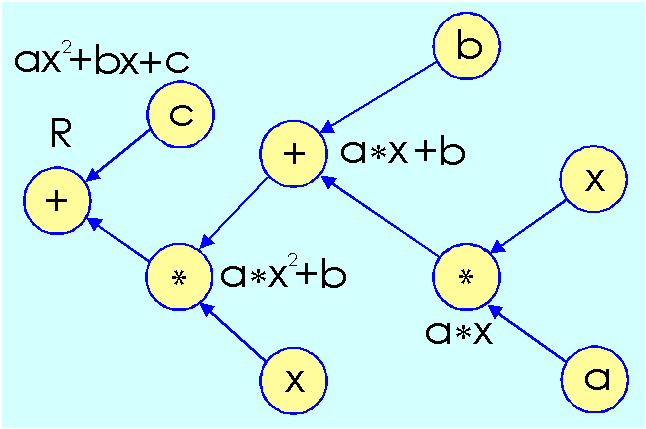
\includegraphics[height=8cm]{img/CalcGraphExample.png}
\end{frame}

\begin{frame}{Фазы выполнения программы}
  \framesubtitle{что это значит}
   
  \begin{columns}
    \column{.7\textwidth}
        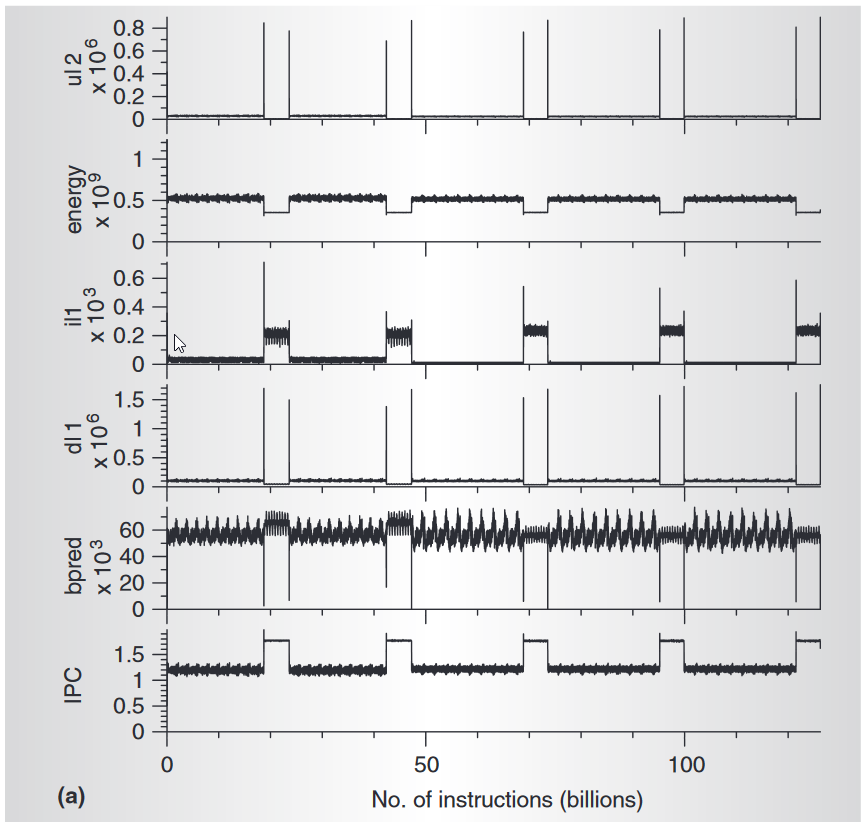
\includegraphics[height=.9\textheight]{img/Phases.png}

    \column{.3\textwidth}
      imothy Sherwood, Erez Perelman, Greg Hamerly, Suleyman Sair, and Brad Calder, Discovering and Exploiting Program Phases, IEEE Micro: Micro's Top Picks from Computer Architecture Conferences
      
     % Figure 1.Plot of metrics over billions of instructions executed by the programs
 % gzip with input graphic (a) and gcc with input 166 (b). Each point on the graph
% is an average over 10 million instructions. These graphs plot the number of uni-
% fied L2 cache misses (ul2), energy consumed by the execution of the instruc-
% tions, number of instruction cache misses (il1), number of data cache misses
% (dl1), number of branch mispredicts (bpred), and the average IPC.
  \end{columns}		  
\end{frame}

\begin{frame}{Фазы выполнения программы}
  \framesubtitle{и части кода этой программы}
  Вопрос: как часто разные фазы работы соотвествуют разным циклам (функциям) или группам операторов?
  
  Ответ: 
  \begin{itemize}
      \item В некоторых примерах соответствуют
      \item Всегда можно придумать контрпример
  \end{itemize}
  % TODO: конкретные (не голословные) оценки, см. бенчмарки
  % TODO: визуализация на основе chstone?
  
\end{frame}

\begin{frame}{Фазы выполнения программы}
  \framesubtitle{бенчмарки}
  \begin{table}
    \begin{tabular}{ | p{1.5cm} | p{2cm} | p{1cm} | p{6cm} |}
    \hline
    Программа & долго счит. гнезд & включают ключ. инт. & особенности \\ \hline
    adpcm & 3 & 3 &  \\ \hline
    aes & 3 & 2 &  \\ \hline
    blowfish & 1 & 1 &  \\ \hline
    dfadd & 1 & 1 &  \\ \hline
    dfdiv & 1 & 0 &  \\ \hline
    dfmul & 1 & 1 &  \\ \hline
    dfsin & 1 & 0 &  \\ \hline
    gsm & 1 & 0 &  \\ \hline
    jpeg & 4 & 3 & \\ \hline
    mips & 1 & 1 & \\ \hline
    motion & 2 & 1 &  \\ \hline
    sha & 1 & 1 &  \\ \hline
    \end{tabular} 
    \caption{Результаты поиска ключевых интервалов в бенчмарках CHStone}
    \label{table:CHStoneSimpoints}
\end{table}

\end{frame}

\begin{frame}{Выбор уровня представления программы для анализа}
  \framesubtitle{высокоуроевневое дерево или промежуточные код?}
  
  \begin{itemize}
      \item AST
      \item SSA
  \end{itemize}
  
\end{frame}

\begin{frame}{Эмуляция архитектуры}
  \framesubtitle{}
  
  \begin{itemize}
      \item Высокотоная эмуляция архитектуры процессора возможна
      \item Но только по полному описанию этой архитектуры
      \item что если мы хотим сделать эмулятор для очень грубой оценки времени работы программы?
      \item ПЛИС это не архитектура, а конструктор любой архитектуры
      \item но возможно составить грубую модель времени выполнения, которая будет отдаленно напоминать реконфигурируемую архитектуру обладающую определенными ресурсами
  \end{itemize}
  
\end{frame}

\begin{frame}{ПЛИС как конструктор вычислительного устройства}
  \framesubtitle{из более крупных блоков}
  
  \begin{itemize}
      \item IP-core
      \item тенденция к укрупнению блоков (не уножители и LUT, а целые DSP и др. готовые устройства) 
      \item возможно представить ресурсы ПЛИС как набор функциональных модулей (вычислителей) на которые отображаются вычисления в исходной программе
 \end{itemize}
  
\end{frame}

\begin{frame}{Скорость работы эмуляции архитектуры}
  \framesubtitle{}
  
  \begin{itemize}
      \item медленно
      \item точный анализ (например, анализ алиасов, анализ указателей) медленный
  \end{itemize}

\end{frame}

\begin{frame}{Вектор простых блоков}
  \framesubtitle{Вектор простых блоков}
  
  \begin{itemize}
      \item Статистика по простым блокам, посещенным во время выполнения
      \item Позволяет статистически оценить поведение программы на тестовых данных
      \item Позволяет найти выборку простых блоков (и конкретные моменты во время работы), по которым можно прогнозировать время работы программы в целом
  \end{itemize}
  
\end{frame}

\begin{frame}[fragile]
  \frametitle{Вектор простых блоков}
  
  \begin{lstlisting}[frame=single]
 

  
  T:182:3   :180:3   :177:3   :1068:6   :1069:4   :1070:7   :1071:4   :1074:8   :1072:8   :1075:6   :1073:6   :1076:3   :1077:1   :1063:2   :1064:2   :1066:4   :1067:1   :1065:10      
T:182:2   :180:1   :177:1   :1087:1   :1095:3   :1096:7   :1097:2   :1098:4   :1099:3   :1100:11   :1101:3   :1103:13   :1105:14   :1107:6   :1110:8   :1108:2   :1109:3   :1104:2   :1106:4   :1102:10   :1111:14   :1112:8   :1113:3   :1115:4   :1116:3   :1117:7   :1118:2   :1119:5   
T:1138:385   :1136:154   :1137:461   
T:1138:385   :1136:154   :1137:461   
T:1138:385   :1136:154   :1137:461   
T:1138:385   :1136:154   :1137:461   
T:1138:385   :1136:153   :1137:462   
T:1138:385   :1136:153   :1137:462   
T:1138:384   :1136:154   :1137:462   
\end{lstlisting}
  
  
\end{frame}


\begin{frame}{Simpoints и аналогичные алгоритмы}
  \framesubtitle{}
  
  \begin{itemize}
      \item Простой статистический метод выбора репрезентативных точек во время выполнения
      
  \end{itemize}
  
\end{frame}


\begin{frame}{Проект эмулятора}
  \framesubtitle{}
   
  \begin{columns}
    \column{.3\textwidth}
      \begin{itemize}
        \item набор функциональных модулей
        \item связи между ними
        \item оценка времени работы при интерпретации
      \end{itemize}

    \column{.7\textwidth}
      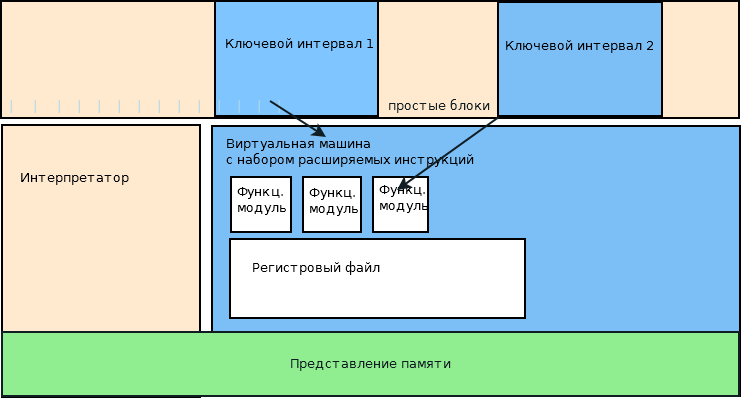
\includegraphics[width=.8\textwidth]{img/Emulator.png}
  \end{columns}		  
\end{frame}

\begin{frame}{Обфускатор}
  \framesubtitle{}
   
  \begin{columns}
    \column{.3\textwidth}
      \begin{itemize}
        \item виртуальная машина со своим набором инструкций
        \item снижение производительности
        \item выполняет другую функцию, но построена по тому же принципу
      \end{itemize}

    \column{.7\textwidth}
      замена инструкций или групп инструкций LLVM на эквивалентные
  \end{columns}		  
\end{frame}

\begin{frame}{Проект эмулятора - текущие результаты}
  \framesubtitle{}
  
  \begin{itemize}
      \item Прототип на LLVM
      \item Интерпретатор
  \end{itemize}
  
\end{frame}

\begin{frame}[allowframebreaks]
        \frametitle{References}
        \bibliographystyle{amsalpha}
        \bibliography{references.bib}
\end{frame}

\end{document}